
\chapter{Diseño de clases} \label{cap:diseño_clases}

\section{Introducción}

% En este capítulo se realizará una breve introducción sobre el diagrama de clases y posteriormente, un análisis de las clases que participan en el modelo de información del simulador. Para ello, se especificarán los atributos, métodos y las relaciones existentes entre las mismas, terminándose con un diagrama de clases general de todo el sistema.



% El propósito de un diagrama de clases es el de representar los objetos fundamentales del sistema, es decir, los que percibe el usuario y con los que espera tratar para completar su tarea. Una clase define el ámbito de definición de un conjunto de objetos.

% Cada clase se representa en un rectángulo con tres apartados:
% \begin{itemize}
% \item Nombre de la clase.

% \item Atributos de la clase.

% \item Operaciones de la clase.
% \end{itemize}


\section{Clases del sistema}

% Según el análisis del sistema realizado hasta ahora,las clases \textbf{principales} que componen el sistema son las siguientes:

% \begin{itemize}
%  \item SimAS.
%  \item Editor.
%  \item Simulador.
%  \item Ayuda.
%  \item Tutorial.
 
% \end{itemize}

% Las clases que serán utilizadas por la clase \textbf{Editor} son las siguientes:

% \begin{itemize}
%  \item Gramatica.
%  \item Produccion.
%  \item Consecuente.
%  \item Antecedente.
%  \item NoTerminal.
%  \item Terminal.
%  \item Simbolo.
%  \item TablaPredictiva.
%  \item TablaLR.
%  \item ParteIrA.
%  \item ParteAccion.
%  \item FuncionesError.
%  \item ColCanLR(0).
%  \item ColCanLR(1).
%  \item ColCanLALR(1).
%  \item ConjElementosLR(0).
%  \item ConjElementosLR(1).
%  \item ConjElementosLALR(1).
%  \item ElementosLR(0).
%  \item ElementosLR(1).
%  \item ElementosLALR(1).

% \end{itemize}

% Las clases que serán utilizadas por la clase \textbf{Simulador} son las siguientes:
 
%  \begin{itemize}
%  \item Gramática.
%  \item CadenaEntrada.
%  \end{itemize}
 
%  Las clases que se encuentran contenidas dentro de la clase \textbf{Ayuda} son las siguientes:
 
%  \begin{itemize}
%   \item Capítulo.
%  \end{itemize}
 
%  Las clases que se encuentran contenidas dentro de la clase \textbf{Tutorial} son las siguientes:

% \begin{itemize}
%  \item Lección.
% \end{itemize}


% A continuación se hará un análisis de cada una de las clases que se han definido anteriormente.

% \subsection{Clase SimAS}

% Esta clase representa a la clase principal del Sistema y es la que se encarga de inicializar los demás componentes de la aplicación. En la tabla \ref{tabla81} se recoge la especificación de la clase
% y en la figura \ref{clase1} se muestra su representación gráfica.

% \begin{longtable}[H]{|>{\columncolor[rgb]{0.63,0.79,0.95}}m{6cm} | m{8.5cm} |}
%  \caption{Clase SimAS}

% \endfirsthead

% \multicolumn{2}{c}
% {{\tablename\ \thetable{} -- continúa de la página anterior}} \\
% \endhead

% \hline \multicolumn{2}{|r|}{{Continúa en la página siguiente}} \\ \hline
% \endfoot

% \hline
% \endlastfoot

% \hline
%  \textbf{Nombre} & \textbf{SimAS}  \\ \hline
 
%  \textbf{Descripción} & Representa la clase principal del simulador.  \\ \hline
                       
%  \textbf{Atributos} & No posee ningún atributo. \\ \hline
 
%  \textbf{Métodos} & \begin{enumerate}
%                 	\item \textbf{init}: método público que permite \textit{inicializar} los componentes 										de la aplicación.
%                 	\item \textbf{lanzarEditor}: método público que permite \textit{lanzar} el módulo Editor del 								simulador.
%                 	\item \textbf{lanzarSimulador}: método público que permite \textit{lanzar} el módulo Simulador del 						simulador.
%                 	\item \textbf{lanzarAyuda}: método público que permite \textit{lanzar} el módulo Ayuda del 								simulador.
%                 	\item \textbf{lanzarTutorial}: método público que permite \textit{lanzar} el módulo Tutorial del 							simulador.
%              \end{enumerate}   
%  \label{tabla81}

% \end{longtable}

%  \begin{figure}[H]
%       \begin{center} 
% 	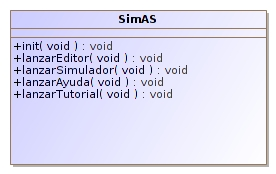
\includegraphics[scale=0.7]{figuras/Cap9/clase1.jpg}
% 	\caption{Representación gráfica de la clase SimAS.}
% 	\label{clase1}
%       \end{center}
%   \end{figure}
  
% \subsection{Clase Editor}

% Esta clase representa al editor de gramáticas y es la que se encarga de editar las gramáticas de contexto
% libre. En la tabla \ref{tabla82} se recoge la especificación de la clase y en la figura \ref{clase2} se muestra su representación gráfica.
  
  
%   \begin{longtable}[H]{|>{\columncolor[rgb]{0.63,0.79,0.95}}m{6cm} | m{8.5cm} |}
%  \caption{Clase Editor}

% \endfirsthead

% \multicolumn{2}{c}
% {{\tablename\ \thetable{} -- continúa de la página anterior}} \\
% \endhead

% \hline \multicolumn{2}{|r|}{{Continúa en la página siguiente}} \\ \hline
% \endfoot

% \hline
% \endlastfoot

% \hline
%  \textbf{Nombre} & \textbf{Editor}  \\ \hline
 
%  \textbf{Descripción} & Representa a un editor de gramáticas.  \\ \hline
                       
%  \textbf{Atributos} & \begin{enumerate}
%  		\item \textbf{gramatica}: instancia de una \textit{gramática} que podrá ser utilizada por el editor. 
%        \end{enumerate}  \\ \hline
 
%  \textbf{Métodos} & \begin{enumerate}
% 		\item \textbf{cargarGramatica}: método público que permite cargar una gramática desde un archivo.
% 		\item \textbf{grabarGramatica}: método público que permite grabar una gramática en un fichero.
% 		\item \textbf{crearGramatica}: método público que permite la creación de una nueva gramática.
% 		\item \textbf{getGramatica}: método público que permite obtener una gramática.
% 		\item \textbf{setGramatica}: método público que permite editar una gramática.
% 		\item \textbf{actualizarVisualizacion}: método privado que permite actualizar la	visualización de la 						gramática en el editor.
%         \end{enumerate}
                                 
%  \label{tabla82}

% \end{longtable}

%  \begin{figure}[H]
%       \begin{center} 
% 	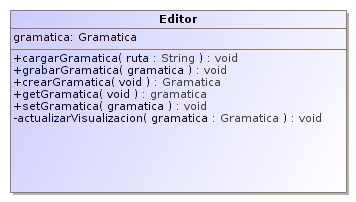
\includegraphics[scale=0.6]{figuras/Cap9/clase2.jpg}
% 	\caption{Representación gráfica de la clase Editor.}
% 	\label{clase2}
%       \end{center}
%   \end{figure}

% \subsection{Clase Gramatica}

% Esta clase representa a las gramáticas de contexto libre. En la tabla \ref{tabla83}
% se recoge la especificación de la clase y en la figura \ref{clase3} se muestra
% su representación gráfica.

% \begin{longtable}[H]{|>{\columncolor[rgb]{0.63,0.79,0.95}}m{6cm} | m{8.5cm} |}
%  \caption{Clase Gramatica}

% \endfirsthead

% \multicolumn{2}{c}
% {{\tablename\ \thetable{} -- continúa de la página anterior}} \\
% \endhead

% \hline \multicolumn{2}{|r|}{{Continúa en la página siguiente}} \\ \hline
% \endfoot

% \hline
% \endlastfoot

% \hline
%  \textbf{Nombre} & \textbf{Gramatica}  \\ \hline
 
%  \textbf{Descripción} & Representa a las gramáticas de contexto libre.  \\ \hline
                       
%  \textbf{Atributos} & \begin{enumerate}
%  		\item \textbf{nombre}: este atributo representa el nombre de la gramática de contexto libre.
%  		\item \textbf{terminales}: este atributo representa el conjunto de símbolos terminales.
%  		\item \textbf{noTerminales}: este atributo representa el conjunto de símbolos no terminales.
% 		 \item \textbf{producciones}: este atrobito representa el conjunto de producciones de la gramática.
% 		 \item \textbf{descripcion}: este atributo representa la descripción de la gramática.
%  		 \item \textbf{TPredictiva}: este atributo representa la tabla predictiva de la gramática.
% \end{enumerate}\\ \hline
	
%  \textbf{Atributos} & \begin{enumerate}
% 		\setcounter{enumi}{6}

% 		 \item \textbf{TLR}: este atributo representa la tabla LR de la gramática.
% 		 \item \textbf{coleccionLR0}: este atributo representa la colección canónica de elementos LR(0).
% 		 \item \textbf{coleccionLR1}: este atributo representa la colección canónica de elementos LR(1).
%  		 \item \textbf{coleccionLALR1}: este atributo representa la colección canónica de elementos LALR(1).
% 		\end{enumerate} \\ \hline
 
%  \textbf{Métodos} & \begin{enumerate}
%  		\item \textbf{getNombre}: método público que permite obtener el nombre de la gramática de contexto libre.
%  		\item \textbf{setNombre}: método público que permite editar el nombre de la gramática de contexto libre.
%  		\item \textbf{getVocabulario}: método público que permite obtener el vocabulario (símbolos terminales y no 				terminales) de una gramática.
% 		\item \textbf{setVocabulario}: método público que permite editar el vocabulario (símbolos terminales y no 				terminales) de una gramática.
% 		\item \textbf{crearSimbolo}: método público que permite crear un símbolo de la gramática, terminal o no 					terminal.
		
% 			\end{enumerate}\\ \hline
	
% 	 \textbf{Métodos} & \begin{enumerate}
% 		\setcounter{enumi}{5}
% 		\item \textbf{eliminarSimbolo}: método público que permite eliminar un símbolo de la gramática, terminal o 				no terminal. Al eliminar un símbolo automáticamente se eliminarán las producciones en las que aparezca 				éste.
% 		\item \textbf{crearProduccion}: método público que permite añadir el antecedente y el consecuente de una 					producción.
% 		\item \textbf{getProduccion}: método público que permite obtener la producción, esto es, el antecedente y el 			consecuente.
				
% 		\item \textbf{setProduccion}: método público que permite editar el antecedente, el consecuente o ambos de 			un producción.
% 		\item \textbf{eliminarProducción}: método público que permite eliminar una producción, esto es, tanto el 					antecedente como el consecuente.
% 		\item \textbf{getDescripcion}: método público que permite obtener la descripción de la gramática.
% 		\item \textbf{setDescripcion}: método público que permite editar la descripción de la gramática.
% 		\item \textbf{generarInforme}: método público que permite generar un informe PDF de la gramática.
% 		\item \textbf{selecSimboloInicial}: método público que permite seleccionar el símbolo inicial de la 						gramática.
		
% 		\end{enumerate}\\ \hline
	
% 	 \textbf{Métodos} & \begin{enumerate}
% 		\setcounter{enumi}{14}
% 		\item \textbf{getSimboloInicial}: método público que permite obtener el símbolo inicial de la gramática.
% 		\item \textbf{transferirGramatica}: método público que permite transferir la	gramática al simulador.
% 		\item \textbf{validarGramatica}: método público que permite validar la gramática.
			
% 		\item \textbf{generarConjPrim}: método público que permite generar el conjunto Primero de la 								gramática.
% 		\item \textbf{getConjPrim}: método público que permite obtener el conjunto primero de la gramática.
% 		\item \textbf{generarConjSig}: método público que permite generar el conjunto Siguiente de la 							gramática.
% 		\item \textbf{getConjSig}: método público que permite obtener el conjunto siguiente de la gramática.
% 		\item \textbf{generarTPredictiva}: método público que permite generar la tabla predictiva para realizar el 				análisis sintáctico descendente.
% 		\item \textbf{getTPredictiva}: método público que permite obtener la tabla predictiva de la gramática.
% 		\item \textbf{generarTLR}: método público que permite generar la tabla LR para realizar el análisis 						sintáctico ascendente.
% 		\item \textbf{getTLR}: método público que permite obtener la tabla LR de la gramática.
		
% 		\end{enumerate}\\ \hline
	
% 	 \textbf{Métodos} & \begin{enumerate}
% 		\setcounter{enumi}{25}
% 		\item \textbf{generarColCanLR0}: método público que permite generar la colección canónica de elementos 					LR(0).
% 		\item \textbf{getColCanLR0}: método método público que permite obtener la colección canónica LR(0) de la 					gramática.
% 		\item \textbf{generarColCanLR1}: método público que permite generar la colección canónica de elementos 					LR(1).
% 		\item \textbf{getColCanLR1}: método público que permite obtener la colección canónica LR(1) de la gramática.
% 		\item \textbf{generarColCanLALR1}: método público que permite generar la colección canónica de elementos 					LALR(1).
% 		\item \textbf{getColCanLALR1}: método público que permite obtener la colección canónica LALR(1) de la 					gramática.
%       \end{enumerate}
                                 
%  \label{tabla83}

% \end{longtable}


% \begin{figure}[H]
%       \begin{center} 
% 	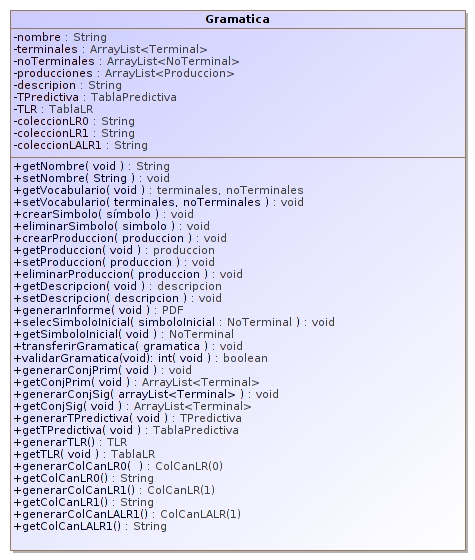
\includegraphics[scale=0.7]{figuras/Cap9/clase3.jpg}
% 	\caption{Representación gráfica de la clase Gramatica.}
% 	\label{clase3}
%       \end{center}
%   \end{figure}

% \subsection{Clase Simbolo}

% Esta clase representa a cualquier símbolo de la gramática (terminal o no terminal). En la tabla \ref{tabla84} se recoge la especificación de la clase y en la figura \ref{clase4} se muestra
% su representación gráfica.
% \newpage

% \begin{longtable}[H]{|>{\columncolor[rgb]{0.63,0.79,0.95}}m{6cm} | m{8.5cm} |}
%  \caption{Clase Simbolo}

% \endfirsthead

% \multicolumn{2}{c}
% {{\tablename\ \thetable{} -- continúa de la página anterior}} \\
% \endhead

% \hline \multicolumn{2}{|r|}{{Continúa en la página siguiente}} \\ \hline
% \endfoot

% \hline
% \endlastfoot

% \hline
%  \textbf{Nombre} & \textbf{Simbolo}  \\ \hline
 
%  \textbf{Descripción} & Representa a cualquier símbolo de la gramática.  \\ \hline
                       
%  \textbf{Atributos} & \begin{enumerate}
%  		\item \textbf{nombre}: \textit{nombre} del símbolo. Si no es un carácter especial, contendrá la 					representación del símbolo.
%  		\item \textbf{valor}: este atributo almacena la \textit{representación} del símbolo (el código 					unicode en caso de que el símbolo fuera especial, como $ \epsilon $).
% 	\end{enumerate} \\ \hline
 
%  \textbf{Métodos}& \begin{enumerate}
%  		\item \textbf{getNombre}: método público que permite obtener el nombre del símbolo. 
% 		 \item \textbf{getValor}: método público que permite obtener el valor del símbolo. 
%  		\item \textbf{setNombre}: método público que permite asignar el nombre del símbolo. 
%  		\item \textbf{setValor}: método público que permite asignar el valor del 	símbolo. 
 		
% 		\end{enumerate}
                                 
%  \label{tabla84}

% \end{longtable}

%  \begin{figure}[H]
%       \begin{center} 
% 	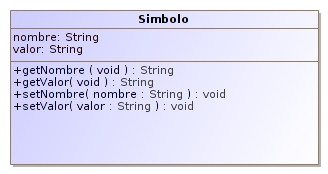
\includegraphics[scale=0.7]{figuras/Cap9/clase4.jpg}
% 	\caption{Representación gráfica de la clase Simbolo.}
% 	\label{clase4}
%       \end{center}
%   \end{figure}
  
% \subsection{Clase Terminal}

% Esta clase representa a cualquier símbolo terminal de la gramática, la cual hereda todos los atributos y métodos de la clase Símbolo. En la tabla \ref{tabla85}
% se recoge la especificación de la clase y en la figura \ref{clase5} se muestra
% su representación gráfica.

% \begin{longtable}[H]{|>{\columncolor[rgb]{0.63,0.79,0.95}}m{6cm} | m{8.5cm} |}
%  \caption{Clase Terminal}

% \endfirsthead

% \multicolumn{2}{c}
% {{\tablename\ \thetable{} -- continúa de la página anterior}} \\
% \endhead

% \hline \multicolumn{2}{|r|}{{Continúa en la página siguiente}} \\ \hline
% \endfoot

% \hline
% \endlastfoot

% \hline
%  \textbf{Nombre} & \textbf{Terminal}  \\ \hline
 
%  \textbf{Descripción} & Representa a los símbolos terminales de la gramática.  \\ \hline
                       
%  \textbf{Atributos} & Hereda los atributos de la clase Símbolo. \\ \hline
 
%  \textbf{Métodos} & Hereda los métodos de la clase Símbolo.
                                 
%  \label{tabla85}

% \end{longtable}

%  \begin{figure}[H]
%       \begin{center} 
% 	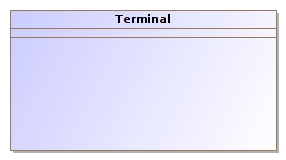
\includegraphics[scale=0.6]{figuras/Cap9/clase5.jpg}
% 	\caption{Representación gráfica de la clase Terminal.}
% 	\label{clase5}
%       \end{center}
%   \end{figure}


% \subsection{Clase NoTerminal}

% Esta clase representa a cualquier símbolo no terminal de la gramática, la cual hereda todos los atributos y métodos de la clase Símbolo. En la tabla \ref{tabla86} se recoge la especificación de la clase y en la figura \ref{clase6} se muestra su representación gráfica.

% \newpage

% \begin{longtable}[H]{|>{\columncolor[rgb]{0.63,0.79,0.95}}m{6cm} | m{8.5cm} |}
%  \caption{Clase NoTerminal}

% \endfirsthead

% \multicolumn{2}{c}
% {{\tablename\ \thetable{} -- continúa de la página anterior}} \\
% \endhead

% \hline \multicolumn{2}{|r|}{{Continúa en la página siguiente}} \\ \hline
% \endfoot

% \hline
% \endlastfoot

% \hline
%  \textbf{Nombre} & \textbf{NoTerminal}  \\ \hline
 
%  \textbf{Descripción} & Representa a los símbolos no terminales de la gramática.  \\ \hline
                       
%  \textbf{Atributos} & \begin{enumerate}
%  		 \item \textbf{simboloInicial}: indica si el símbolo no terminal es inicial o no.
%  		 \item \textbf{primeros}: lista de símbolos terminales que forman el conjunto primero del símbolo terminal, 				también 	puede contener $\epsilon$.
%  		 \item \textbf{siguientes}: lista de símbolos terminales que forman el conjunto siguiente del símbolo 					no terminal, también puede contener \$.
% 		\end{enumerate}  \\ \hline
 
%  \textbf{Métodos} & \begin{enumerate}
%  		\item \textbf{getSimInicial}: método público que \textit{devuelve} si el símbolo es inicial o no.
%  		\item \textbf{setSimInicial}: método público que \textit{permite asignar} el valor 1 si el símbolo terminal 				es el símbolo	inicial y el valor 0 en el caso contrario.
%  		\item \textbf{getPrimeros}: método público que \textit{devuelve} el conjunto Primero del símbolo no 						terminal.
%  		\item \textbf{setPrimeros}: método público que permite almacenar la lista de símbolos terminales 							que forman parte del conjunto Primero.
%  		\item \textbf{getSiguientes}: método público que devuelve el conjunto Siguiente del símbolo no 							terminal.
%  			\end{enumerate}\\ \hline
	
%  \textbf{Métodos} & \begin{enumerate}
% 		\setcounter{enumi}{5}
 		
%  		\item \textbf{setSiguientes}: método público que permite almacenar la lista de símbolos terminales 						que 	forman parte del conjunto Siguiente.
 
%  		\end{enumerate}
                                 
%  \label{tabla86}

% \end{longtable}

%  \begin{figure}[H]
%       \begin{center} 
% 	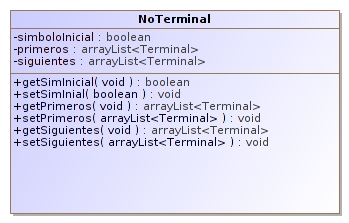
\includegraphics[scale=0.6]{figuras/Cap9/clase6.jpg}
% 	\caption{Representación gráfica de la clase NoTerminal.}
% 	\label{clase6}
%       \end{center}
%   \end{figure}


% \subsection{Clase Produccion}

% Esta clase representa a las producciones de la gramática. En la tabla \ref{tabla88} se recoge la especificación de la clase y en la figura \ref{clase8} se muestra su representación gráfica.

% \begin{longtable}[H]{|>{\columncolor[rgb]{0.63,0.79,0.95}}m{6cm} | m{8.5cm} |}
%  \caption{Clase Produccion}

% \endfirsthead

% \multicolumn{2}{c}
% {{\tablename\ \thetable{} -- continúa de la página anterior}} \\
% \endhead

% \hline \multicolumn{2}{|r|}{{Continúa en la página siguiente}} \\ \hline
% \endfoot

% \hline
% \endlastfoot

% \hline
%  \textbf{Nombre} & \textbf{Produccion}  \\ \hline
 
%  \textbf{Descripción} & Representa a los producciones de la gramática.  \\ \hline
                       
%  \textbf{Atributos} & \begin{enumerate}
%  		\item \textbf{antec}: representa al \textit{antecedente} de la producción (símbolo no 								terminal).
%  		\item \textbf{consec}: representa al \textit{consecuente} de la producción (que es una lista de 						símbolos terminales y no terminales, o lo que es lo mismo, de símbolos gramaticales). También puede ser 				el símbolo $\epsilon$.
% 		\end{enumerate}\\ \hline
 
%  \textbf{Métodos} & \begin{enumerate}
%  		\item \textbf{getAntecedente}: método público que devuelve el antecedente de una producción.
%  		\item \textbf{setAntecedente}: método público que permite almacenar el antecedente de una producción.
%  		\item \textbf{getConsecuente}: método público que devuelve el consecuente de una producción.
%  		\item \textbf{setConsecuente}: método público que permite almacenar el consecuente de una producción. 

% \end{enumerate}
                                 
%  \label{tabla88}

% \end{longtable}

%  \begin{figure}[H]
%       \begin{center} 
% 	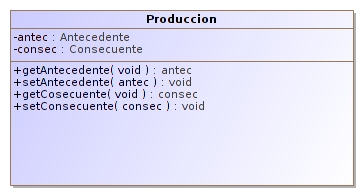
\includegraphics[scale=0.6]{figuras/Cap9/clase8.jpg}
% 	\caption{Representación gráfica de la clase Produccion.}
% 	\label{clase8}
%       \end{center}
%   \end{figure}

% \subsection{Clase Antecedente}

% Esta clase representa al antecedente de la producción de una gramática. En la tabla \ref{tabla89} se recoge la especificación de la clase y en la figura \ref{clase9} se muestra su representación gráfica.

% \begin{longtable}[H]{|>{\columncolor[rgb]{0.63,0.79,0.95}}m{6cm} | m{8.5cm} |}
%  \caption{Clase Antecedente}

% \endfirsthead

% \multicolumn{2}{c}
% {{\tablename\ \thetable{} -- continúa de la página anterior}} \\
% \endhead

% \hline \multicolumn{2}{|r|}{{Continúa en la página siguiente}} \\ \hline
% \endfoot

% \hline
% \endlastfoot

% \hline
%  \textbf{Nombre} & \textbf{Antecedente}  \\ \hline
 
%  \textbf{Descripción} & Representa al antecedente de una producción.  \\ \hline
                       
%  \textbf{Atributos} & \begin{enumerate}
%  		\item \textbf{simboloNT}: representa el símbolo no terminal que forma parte del antecedente de una 						producción.
%  		\end{enumerate} \\ \hline
 
%  \textbf{Métodos} & \begin{enumerate}
%   		\item \textbf{getSimboloNT}: método público que permite obtener el símbolo no terminal que forma parte del 				antecedente de la producción.
%   		\item \textbf{setSimboloNT}: método público que permite asignar un símbolo no terminal de la gramática 					definida al	antecedente de la producción.
%   \end{enumerate}
                                
%  \label{tabla89}

% \end{longtable}

%  \begin{figure}[H]
%       \begin{center} 
% 	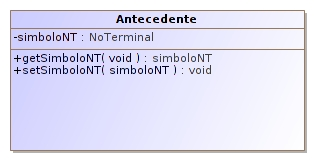
\includegraphics[scale=0.6]{figuras/Cap9/clase9.jpg}
% 	\caption{Representación gráfica de la clase Antecedente.}
% 	\label{clase9}
%       \end{center}
%   \end{figure}

% \subsection{Clase Consecuente}

% Esta clase representa al consecuente de la producción de una gramática. En la tabla \ref{tabla810} se recoge la especificación de la clase y en la figura \ref{clase10} se muestra su representación gráfica.

% \begin{longtable}[H]{|>{\columncolor[rgb]{0.63,0.79,0.95}}m{6cm} | m{8.5cm} |}
%  \caption{Clase Consecuente}

% \endfirsthead

% \multicolumn{2}{c}
% {{\tablename\ \thetable{} -- continúa de la página anterior}} \\
% \endhead

% \hline \multicolumn{2}{|r|}{{Continúa en la página siguiente}} \\ \hline
% \endfoot

% \hline
% \endlastfoot

% \hline
%  \textbf{Nombre} & \textbf{Consecuente}  \\ \hline
 
%  \textbf{Descripción} & Representa al consecuente de una producción.  \\ \hline
                       
%  \textbf{Atributos} & \begin{enumerate}
%     		\item \textbf{conjSimbolos}: representa al \textit{consecuente} de la producción (que es una lista de 					símbolos terminales y no terminales, o lo que es lo mismo, de símbolos gramaticales). También puede ser 				el símbolo $\epsilon$.
%  \end{enumerate} \\ \hline
 
%  \textbf{Métodos} & \begin{enumerate}
%   		\item \textbf{getconjSimbolos}: método público que permite obtener el conjunto de símbolos que componen el 				consecuente de la producción.
%   		\item \textbf{setconjSimbolos}: método público que permite asignar el conjunto de símbolos al consecuente de 			la producción.
%   \end{enumerate}
                                 
%  \label{tabla810}

% \end{longtable}

%  \begin{figure}[H]
%       \begin{center} 
% 	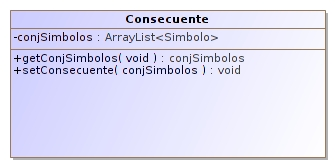
\includegraphics[scale=0.6]{figuras/Cap9/clase10.jpg}
% 	\caption{Representación gráfica de la clase Consecuente.}
% 	\label{clase10}
%       \end{center}
%   \end{figure}



% \subsection{Clase TablaPredictiva}

% Esta clase representa a la tabla Predictiva de una gramática de contexto libre. En la tabla \ref{tabla812}
% se recoge la especificación de la clase y en la figura \ref{clase12} se muestra su representación gráfica.

% \begin{longtable}[H]{|>{\columncolor[rgb]{0.63,0.79,0.95}}m{6cm} | m{8.5cm} |}
%  \caption{Clase TablaPredictiva}

% \endfirsthead

% \multicolumn{2}{c}
% {{\tablename\ \thetable{} -- continúa de la página anterior}} \\
% \endhead

% \hline \multicolumn{2}{|r|}{{Continúa en la página siguiente}} \\ \hline
% \endfoot

% \hline
% \endlastfoot

% \hline
%  \textbf{Nombre} & \textbf{TablaPredictiva}  \\ \hline
 
%  \textbf{Descripción} & Representa a la tabla predictiva de una gramática de contexto libre.  \\ \hline
                       
%  \textbf{Atributos} & \begin{enumerate}
%  		\item \textbf{funError}: representa las funciones de tratamiento de errores para completar la tabla 						predictiva.
%  		\item \textbf{matrizPred}: este atributo representa la matriz predictiva. La matriz tendrá las siguientes 				dimensiones: [Número de símbolos no terminales] [Número de símbolos terminales + 1 (Símbolo \$)] . Los 				datos dentro de la matriz predictiva pueden ser de dos tipos: 
%  			\begin{itemize}
% 				\item \textit{PN}: producción número \textit{N}.
% 				\item \textit{EN}: función de error número \textit{N}.
% 			\end{itemize}
%  		\end{enumerate}  \\ \hline
 
%  \textbf{Métodos} & \begin{enumerate}
%  		\item \textbf{construir}: método público que permite construir la tabla Predictiva.
%  		\item \textbf{getCeldaPredictiva}: método público que permite obtener una celda de la matriz de la tabla 					predictiva. 		
%  		\item \textbf{setCeldaPredictiva}: método público que permite asignar un valor a una celda de la matriz de 				la tabla predictiva.	
%  		\item \textbf{crearFunError}: método público que permite crear una nueva función de error.
%  		\item \textbf{asignarFuncionError}: método público que permite asignar las funciones de tratamiento de error 			a la tabla.
%  		\item \textbf{editarFucionError}: método público que permite editar un función de error.
%  		\item \textbf{eliminarFunError}: método público que permite eliminar una función de error ya creada. Si se 				elimina una función que ya está asignada en la tabla se eliminará dicha asignación.
% \end{enumerate}
                                 
%  \label{tabla812}

% \end{longtable}

%  \begin{figure}[H]
%       \begin{center} 
% 	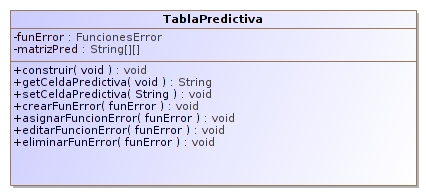
\includegraphics[scale=0.6]{figuras/Cap9/clase12.jpg}
% 	\caption{Representación gráfica de la clase TablaPredictiva.}
% 	\label{clase12}
%       \end{center}
%   \end{figure}


% \subsection{Clase TablaLR}

% Esta clase representa a la tabla LR de una gramática de contexto libre. En la tabla \ref{tabla813} se recoge la especificación de la clase y en la figura \ref{clase13} se muestra su representación gráfica.

% \begin{longtable}[H]{|>{\columncolor[rgb]{0.63,0.79,0.95}}m{6cm} | m{8.5cm} |}
%  \caption{Clase TablaLR}

% \endfirsthead

% \multicolumn{2}{c}
% {{\tablename\ \thetable{} -- continúa de la página anterior}} \\
% \endhead

% \hline \multicolumn{2}{|r|}{{Continúa en la página siguiente}} \\ \hline
% \endfoot

% \hline
% \endlastfoot

% \hline
%  \textbf{Nombre} & \textbf{TablaLR}  \\ \hline
 
%  \textbf{Descripción} & Representa a la tabla LR de una gramática de con\-tex\-to libre.  \\ \hline
                       
%  \textbf{Atributos} & \begin{enumerate}
% 	 \item \textbf{metodoAscendente}: este tipo enumerado representa a los métodos de simulación del 							análisis sintáctico ascendente que pueden ser utilizados en el simulador (SLR, LR, LALR).
% 	 \item \textbf{TAccion}: este atributo representa a la tabla de la parte acción del análisis.
% 	 \item \textbf{TIrA}: este atributo representa a la tabla de la parte ir\_a del análisis.
 	
% 	\end{enumerate} \\ \hline
 
%  \textbf{Métodos} & \begin{enumerate}
%  	 \item \textbf{getMetodoAsc}: método público que obtiene el valor del método ascendente.
%  	 \item \textbf{setMetodoAsc}: método público que permite almacenar el valor del método ascendente.
%  	 \item \textbf{generarAccion}: método público que permite construir la parte acción de la tabla LR en función 				del método seleccionado.
%  	 \item \textbf{getAccion}: método público que permite obtener la matriz acción de la gramática.
%  	 \item \textbf{generarIrA}: método público que permite construir la parte ir\_A de la tabla LR en función 				del método seleccionado.
%  	 \item \textbf{getIrA}: método público que permite obtener la matriz Ir\_A de la gramática.
% 	\end{enumerate}
                                 
%  \label{tabla813}

% \end{longtable}

%  \begin{figure}[H]
%       \begin{center} 
% 	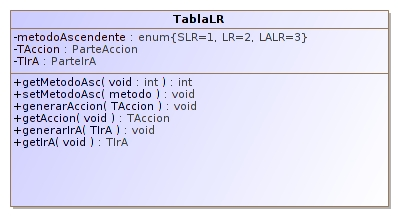
\includegraphics[scale=0.6]{figuras/Cap9/clase13.jpg}
% 	\caption{Representación gráfica de la clase TablaLR.}
% 	\label{clase13}
%       \end{center}
%   \end{figure}
  
% \subsection{Clase ParteAccion}

% Esta clase representa a la parte acción de la tabla LR de una gramática de contexto libre. En la tabla \ref{tabla819} se recoge la especificación de la clase y en la figura \ref{clase19} se muestra su representación gráfica.

% \begin{longtable}[H]{|>{\columncolor[rgb]{0.63,0.79,0.95}}m{6cm} | m{8.5cm} |}
%  \caption{Clase ParteAccion}

% \endfirsthead

% \multicolumn{2}{c}
% {{\tablename\ \thetable{} -- continúa de la página anterior}} \\
% \endhead

% \hline \multicolumn{2}{|r|}{{Continúa en la página siguiente}} \\ \hline
% \endfoot

% \hline
% \endlastfoot

% \hline
%  \textbf{Nombre} & \textbf{ParteAccion}  \\ \hline
 
%  \textbf{Descripción} & Representa a la parte acción de la tabla LR de una gramática de con\-tex\-to libre.  \\ \hline
                       
%  \textbf{Atributos} &  \begin{enumerate}
%   		\item \textbf{funError}: funciones de tratamiento de errores para completar la tabla predictiva.
%  		\item \textbf{matrizAccion}: representa en forma de matriz la parte acción de una tabla LR. La matriz tendrá 		la siguiente dimensión: [Número de estados + 1] [Número de símbolos terminales + 1 (el símbolo \$)]. Los 				datos dentro de la matriz acción pueden ser de los siguientes tipos: 
%  		\begin{itemize}
% 			\item \textit{A}: aceptar.
% 			\item \textit{RN}: reducir con la producción número \textit{N}.
% 			\item \textit{DN}: desplazar y pasar al estado número \textit{N}.
% 			\item \textit{EN}: función de error número \textit{N}.
% 		\end{itemize}
					

%  		\end{enumerate}  \\ \hline
 
%  \textbf{Métodos} & \begin{enumerate} 
%  		\item \textbf{construir}: método público que permite construir la matriz de la parte Acción.
%  		\item \textbf{getCeldaAccion}: método público que permite obtener una celda de la matriz de la parte Acción. 
 		
%  		\item \textbf{setCeldaAccion}: método público que permite asignar un valor a una celda de la matriz de 				la parte Acción.	
%  		\item \textbf{crearFunError}: método público que permite crear una nueva función de error.
%  		\item \textbf{asignarFuncionError}: método público que permite asignar las funciones de tratamiento de error 			a la tabla.
%  		\item \textbf{editarFucionError}: método público que permite editar un función de error.
%  		\item \textbf{eliminarFunError}: método público que permite eliminar una función de error ya creada. Si se 				elimina una función que ya está asignada en la tabla se eliminará dicha asignación.
% \end{enumerate}
                                 
%  \label{tabla819}

% \end{longtable}

% \begin{figure}[H]
%       \begin{center} 
% 	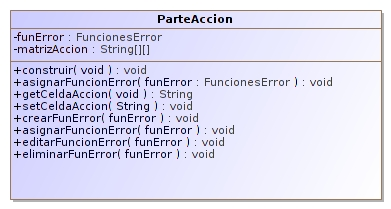
\includegraphics[scale=0.6]{figuras/Cap9/clase19.jpg}
% 	\caption{Representación gráfica de la clase ParteAccion}
% 	\label{clase19}
%       \end{center}
%   \end{figure}


% \subsection{Clase ParteIrA}

% Esta clase representa a la parte ir a de la tabla LR de una gramática de contexto libre. En la tabla \ref{tabla820} se recoge la especificación de la clase y en la figura \ref{clase20} se muestra su representación gráfica.

% \begin{longtable}[H]{|>{\columncolor[rgb]{0.63,0.79,0.95}}m{6cm} | m{8.5cm} |}
%  \caption{Clase ParteIrA}

% \endfirsthead

% \multicolumn{2}{c}
% {{\tablename\ \thetable{} -- continúa de la página anterior}} \\
% \endhead

% \hline \multicolumn{2}{|r|}{{Continúa en la página siguiente}} \\ \hline
% \endfoot

% \hline
% \endlastfoot

% \hline
%  \textbf{Nombre} & \textbf{ParteIrA}  \\ \hline
 
%  \textbf{Descripción} & Representa a la parte ir a de la tabla LR de una gramática de con\-tex\-to libre.  \\ \hline
                       
%  \textbf{Atributos} & \begin{enumerate}
% 		\item \textbf{matrizIrA}: representa en forma de matriz la parte ir\_a de la tabla LR. La matriz tendrá la 				siguiente dimensión: [Número de estados + 1] [Número de simbolos no terminales]. Los datos que 						contiene esta matriz son las transiciones del autómata finito determinista (AFD)
% \end{enumerate} \\ \hline
 
%  \textbf{Métodos} & \begin{enumerate}
% 		\item \textbf{construir}: método público que permite construir la matriz de la parte Ir\_A.
%  		\item \textbf{getCeldaIrA}: método público que permite obtener una celda de la matriz de la parte Acción. 
%  		\item \textbf{setCeldaIrA}: método público que permite asignar un valor a una celda de la matriz de 					la parte Ir\_A.
% 		 \end{enumerate}	
                                 
%  \label{tabla820}

% \end{longtable}

% \begin{figure}[H]
%       \begin{center} 
% 	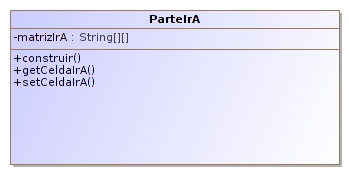
\includegraphics[scale=0.6]{figuras/Cap9/clase20.jpg}
% 	\caption{Representación gráfica de la clase ParteIrA.}
% 	\label{clase20}
%       \end{center}
%   \end{figure}

% \subsection{Clase FuncionError}

% Esta clase representa a las funciones de error utilizadas para completar tanto la tabla predictiva como la tabla LR de una gramática de contexto libre. En la tabla \ref{tabla814} se recoge la especificación de la clase y en la figura \ref{clase14} se muestra su representación gráfica.

% \begin{longtable}[H]{|>{\columncolor[rgb]{0.63,0.79,0.95}}m{6cm} | m{8.5cm} |}
%  \caption{Clase FuncionError}

% \endfirsthead

% \multicolumn{2}{c}
% {{\tablename\ \thetable{} -- continúa de la página anterior}} \\
% \endhead

% \hline \multicolumn{2}{|r|}{{Continúa en la página siguiente}} \\ \hline
% \endfoot

% \hline
% \endlastfoot

% \hline
%  \textbf{Nombre} & \textbf{FuncionError}  \\ \hline
 
%  \textbf{Descripción} & Representa a las funciones de error con las que se completan tanto la tabla 					predictiva como la tabla LR de una gramática de con\-tex\-to libre.  \\ \hline
                       
%  \textbf{Atributos} & \begin{enumerate}
%  		\item \textbf{identificador}: representa al \textit{identificador} de una función de e\-rror.
% 		 \item \textbf{mensaje}: representa al \textit{mensaje} de una función de e\-rror.
%  		\item \textbf{accion}: representa a la \textit{acción} que lle\-va a cabo la función de e\-rror. Habrá que 				diferenciar entre la acción en las funciones de error en el análisis sintáctico ascendente y 							descendente.
%  		\item \textbf{simbolo}: representa al \textit{símbolo} que utiliza la función de e\-rror (tanto en la 			entrada como en la pila) o una \textbf{modificación} (tanto en la entrada como en la pila), que 				consistiría en cambiar un símbolo por otro.

% 	\end{enumerate} \\ \hline
 
%  \textbf{Métodos} & \begin{enumerate}
%  		\item \textbf{getIdentificador}: método público que permite obtener el identificador de la función de error. 
%  		\item \textbf{setIdentificador}: método público que permite asignar el identificador a la función de error.
%  		\item \textbf{getMensaje}: método público que permite obtener el mensaje	de la función de error. 
% 	 	\item \textbf{setMensaje}: método público que permite asignar el mensaje a la función de error.
% 	 	\item \textbf{getAccion}: método público que permite obtener la acción que lleva a cabo la función de error.
%  		\item \textbf{setAccion}: método público que permite asignar la accion a 	la función de error.
% 		\item \textbf{getSimbolo}:método público que permite obtener el simbolo que utiliza la función de error (en 				caso de que utilice alguno).
%  		\item \textbf{setSimbolo}: método público que permite asignar el simbolo a la función de error.

% \end{enumerate}
                             
%  \label{tabla814}

% \end{longtable}

%  \begin{figure}[H]
%       \begin{center} 
% 	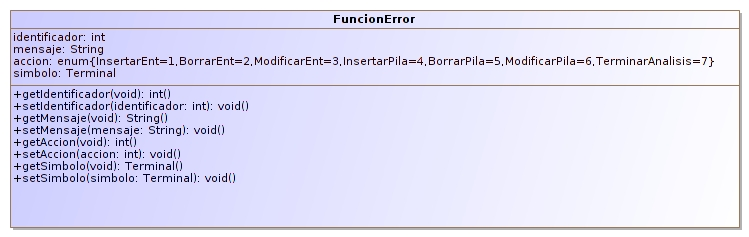
\includegraphics[scale=0.6]{figuras/Cap9/clase14.jpg}
% 	\caption{Representación gráfica de la clase FuncionError.}
% 	\label{clase14}
%       \end{center}
%   \end{figure}
  
% \subsection{ColCanLR(0)}

% Esta clase representa a la colección canónica de elementos LR(0) necesaria para llevar a cabo el análisis sintáctico ascendente SLR. En la tabla \ref{tabla822} se recoge la especificación de la clase y en la figura \ref{clase22} se muestra su representación gráfica.


% \begin{longtable}[H]{|>{\columncolor[rgb]{0.63,0.79,0.95}}m{6cm} | m{8.5cm} |}
%  \caption{Clase ColCanLR(0)}

% \endfirsthead

% \multicolumn{2}{c}
% {{\tablename\ \thetable{} -- continúa de la página anterior}} \\
% \endhead

% \hline \multicolumn{2}{|r|}{{Continúa en la página siguiente}} \\ \hline
% \endfoot

% \hline
% \endlastfoot

% \hline
%  \textbf{Nombre} & \textbf{ColCanLR(0)}  \\ \hline
 
%  \textbf{Descripción} & Representa a colección canónica de elementos LR(0) necesaria en el análisis sintáctica ascendente SLR.  \\ \hline
                       
%  \textbf{Atributos} & \begin{enumerate}
 		
%  		\item \textbf{conjElementosLR0}: este atributo representa el conjunto de elementos LR(0) en el análisis sintáctico ascendente SLR.

% 	\end{enumerate} \\ \hline
 
%  \textbf{Métodos} & \begin{enumerate}
%  		\item \textbf{getConjElementosLR0}: método público que permite obtener el conjunto de elementos LR(0).
%  		\item \textbf{setConjElementosLR0}: método público que permite asignar el valor al conjunto de elementos 					LR(0).

% \end{enumerate}
                             
%  \label{tabla822}

% \end{longtable}

%  \begin{figure}[H]
%       \begin{center} 
% 	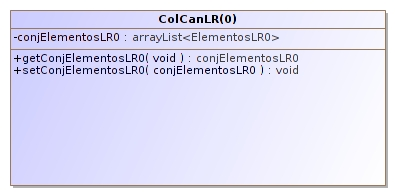
\includegraphics[scale=0.6]{figuras/Cap9/clase22.jpg}
% 	\caption{Representación gráfica de la clase ColCanLR(0).}
% 	\label{clase22}
%       \end{center}
%   \end{figure}

% \subsection{ColCanLR(1)}

% Esta clase representa a la colección canónica de elementos LR(1) necesaria para llevar a cabo el análisis sintáctico ascendente LR-canónico. En la tabla \ref{tabla823} se recoge la especificación de la clase y en la figura \ref{clase823} se muestra su representación gráfica.

% \begin{longtable}[H]{|>{\columncolor[rgb]{0.63,0.79,0.95}}m{6cm} | m{8.5cm} |}
%  \caption{Clase ColCanLR(1)}

% \endfirsthead

% \multicolumn{2}{c}
% {{\tablename\ \thetable{} -- continúa de la página anterior}} \\
% \endhead

% \hline \multicolumn{2}{|r|}{{Continúa en la página siguiente}} \\ \hline
% \endfoot

% \hline
% \endlastfoot

% \hline
%  \textbf{Nombre} & \textbf{ColCanLR(1)}  \\ \hline
 
%  \textbf{Descripción} & Representa a colección canónica de elementos LR(1) necesaria en el análisis sintáctica ascendente LR-canónico.  \\ \hline
                       
%  \textbf{Atributos} & \begin{enumerate}
 		
%  		\item \textbf{conjElementosLR1}: este atributo representa el conjunto de elementos LR(1) en el análisis 					sintáctico ascendente LR-canónico.

% 	\end{enumerate} \\ \hline
 
%  \textbf{Métodos} & \begin{enumerate}
%  		\item \textbf{getConjElementosLR1}: método público que permite obtener el conjunto de elementos LR(1).
%  		\item \textbf{setConjElementosLR1}: método público que permite asignar el valor al conjunto de elementos 					LR(1).
% \end{enumerate}
                             
%  \label{tabla823}

% \end{longtable}

%  \begin{figure}[H]
%       \begin{center} 
% 	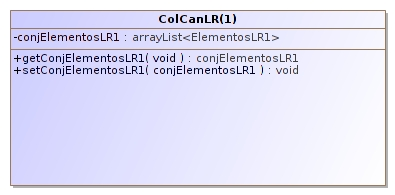
\includegraphics[scale=0.6]{figuras/Cap9/clase23.jpg}
% 	\caption{Representación gráfica de la clase ColCanLR(1).}
% 	\label{clase823}
%       \end{center}
%   \end{figure}


% \subsection{ColCanLALR(1)}

% Esta clase representa a la colección canónica de elementos LALR(1) necesaria para llevar a cabo el análisis sintáctico ascendente LALR. En la tabla \ref{tabla824} se recoge la especificación de la clase y en la figura \ref{clase824} se muestra su representación gráfica.


% \begin{longtable}[H]{|>{\columncolor[rgb]{0.63,0.79,0.95}}m{6cm} | m{8.5cm} |}
%  \caption{Clase ColCanLALR(1)}

% \endfirsthead

% \multicolumn{2}{c}
% {{\tablename\ \thetable{} -- continúa de la página anterior}} \\
% \endhead

% \hline \multicolumn{2}{|r|}{{Continúa en la página siguiente}} \\ \hline
% \endfoot

% \hline
% \endlastfoot

% \hline
%  \textbf{Nombre} & \textbf{ColCanLALR(1)}  \\ \hline
 
%  \textbf{Descripción} & Representa a colección canónica de elementos LALR(1) necesaria en el análisis sintáctica ascendente LALR.  \\ \hline
                       
%  \textbf{Atributos} & \begin{enumerate}
 		
%  		\item \textbf{conjElementosLALR1}: este atributo representa el conjunto de elementos LALR(1) en el análisis 				sintáctico ascendente LALR.

% 	\end{enumerate} \\ \hline
 
%  \textbf{Métodos} & \begin{enumerate}
%  		\item \textbf{getConjElementosLALR1}: método público que permite obtener el conjunto de elementos LALR(1).
%  		\item \textbf{setConjElementosLALR1}: método público que permite asignar el valor al conjunto de elementos 				LALR(1).

% \end{enumerate}
                             
%  \label{tabla824}

% \end{longtable}

%  \begin{figure}[H]
%       \begin{center} 
% 	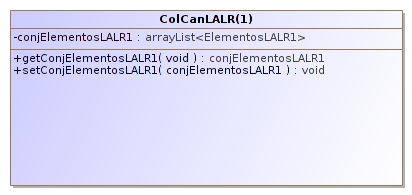
\includegraphics[scale=0.6]{figuras/Cap9/clase24.jpg}
% 	\caption{Representación gráfica de la clase ColCanLALR(1).}
% 	\label{clase824}
%       \end{center}
%   \end{figure}

% \subsection{ConjElementosLR(0)}

% Esta clase representa al conjunto de elementos LR(0) necesaria para llevar a cabo el análisis sintáctico ascendente SLR. En la tabla \ref{tabla825} se recoge la especificación de la clase y en la figura \ref{clase825} se muestra su representación gráfica.

% \begin{longtable}[H]{|>{\columncolor[rgb]{0.63,0.79,0.95}}m{6cm} | m{8.5cm} |}
%  \caption{Clase ConjElementosLR(0)}

% \endfirsthead

% \multicolumn{2}{c}
% {{\tablename\ \thetable{} -- continúa de la página anterior}} \\
% \endhead

% \hline \multicolumn{2}{|r|}{{Continúa en la página siguiente}} \\ \hline
% \endfoot

% \hline
% \endlastfoot

% \hline
%  \textbf{Nombre} & \textbf{ConjElementosLR(0)}  \\ \hline
 
%  \textbf{Descripción} & Representa al conjunto de elementos LR(0) necesaria en el análisis sintáctica ascendente SLR.  \\ \hline
                       
%  \textbf{Atributos} & \begin{enumerate}
%  		\item \textbf{elementosLR0}: este atributo representa al conjunto de todos los elementos LR(0) de la 						gramática. Se utiliza en el análisis sintáctico SLR. 
%  \end{enumerate}\\ \hline
 
%  \textbf{Métodos} & \begin{enumerate}
%  		\item \textbf{getElementosLR0}: método público que permite obtener los elementos LR(0).
%  		\item \textbf{setElementosLR0}: método público que permite asignar el valor al conjunto de elementos LR(0).


% \end{enumerate}
                             
%  \label{tabla825}

% \end{longtable}

%  \begin{figure}[H]
%       \begin{center} 
% 	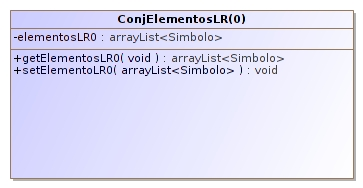
\includegraphics[scale=0.6]{figuras/Cap9/clase25.jpg}
% 	\caption{Representación gráfica de la clase ConjElementosLR(0).}
% 	\label{clase825}
%       \end{center}
%   \end{figure}

% \subsection{ConjElementosLR(1)}

% Esta clase representa al conjunto de elementos LR(1) necesaria para llevar a cabo el análisis sintáctico ascendente LR-canónico. En la tabla \ref{tabla826} se recoge la especificación de la clase y en la figura \ref{clase826} se muestra su representación gráfica.


% \begin{longtable}[H]{|>{\columncolor[rgb]{0.63,0.79,0.95}}m{6cm} | m{8.5cm} |}
%  \caption{Clase ConjElementosLR(1)}

% \endfirsthead

% \multicolumn{2}{c}
% {{\tablename\ \thetable{} -- continúa de la página anterior}} \\
% \endhead

% \hline \multicolumn{2}{|r|}{{Continúa en la página siguiente}} \\ \hline
% \endfoot

% \hline
% \endlastfoot

% \hline
%  \textbf{Nombre} & \textbf{ConjElementosLR(1)}  \\ \hline
 
%  \textbf{Descripción} & Representa al conjunto de elementos LR(1) necesaria en el análisis sintáctica ascendente LR-canónico.  \\ \hline
                       
%  \textbf{Atributos} & \begin{enumerate}
%  		\item \textbf{elementosLR1}: este atributo representa al conjunto de todos los elementos LR(1) de la 						gramática. Se utiliza en el análisis sintáctico LR-canónico.

% 	\end{enumerate} \\ \hline
 
%  \textbf{Métodos} & \begin{enumerate}
%  		\item \textbf{getElementosLR1}: método público que permite obtener los elementos LR(1).
%  		\item \textbf{setElementosLR1}: método público que permite asignar el valor a los elementos LR(1).

% \end{enumerate}
                             
%  \label{tabla826}

% \end{longtable}

%  \begin{figure}[H]
%       \begin{center} 
% 	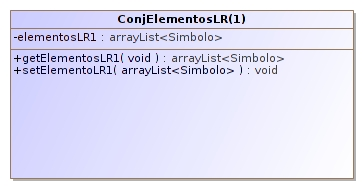
\includegraphics[scale=0.6]{figuras/Cap9/clase26.jpg}
% 	\caption{Representación gráfica de la clase ConjElementosLR(1).}
% 	\label{clase826}
%       \end{center}
%   \end{figure}

% \subsection{ConjElementosLARL(1)}

% Esta clase representa al conjunto de elementos LALR(1) necesaria para llevar a cabo el análisis sintáctico ascendente LALR. En la tabla \ref{tabla827} se recoge la especificación de la clase y en la figura \ref{clase827} se muestra su representación gráfica.


% \begin{longtable}[H]{|>{\columncolor[rgb]{0.63,0.79,0.95}}m{6cm} | m{8.5cm} |}
%  \caption{Clase ConjElementosLALR(1)}

% \endfirsthead

% \multicolumn{2}{c}
% {{\tablename\ \thetable{} -- continúa de la página anterior}} \\
% \endhead

% \hline \multicolumn{2}{|r|}{{Continúa en la página siguiente}} \\ \hline
% \endfoot

% \hline
% \endlastfoot

% \hline
%  \textbf{Nombre} & \textbf{ConjElementosLALR(1)}  \\ \hline
 
%  \textbf{Descripción} & Representa al conjunto de elementos LALR(1) necesaria en el análisis sintáctica ascendente LALR.  \\ \hline
                       
%  \textbf{Atributos} & \begin{enumerate}
%  		\item \textbf{elementosLALR1}: este atributo representa al conjunto de todos los elementos LALR(1) de la 						gramática. Se utiliza en el análisis sintáctico LALR.

% 	\end{enumerate} \\ \hline
 
%  \textbf{Métodos} & \begin{enumerate}
%  		\item \textbf{getElementosLALR1}: método público que permite obtener los elementos LALR(1).
%  		\item \textbf{setElementosLALR1}: método público que permite asignar el valor a los elementos LALR(1).

% \end{enumerate}
                             
%  \label{tabla827}

% \end{longtable}

%  \begin{figure}[H]
%       \begin{center} 
% 	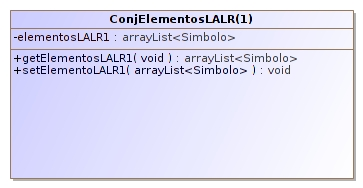
\includegraphics[scale=0.6]{figuras/Cap9/clase27.jpg}
% 	\caption{Representación gráfica de la clase ConjElementosLALR(1).}
% 	\label{clase827}
%       \end{center}
%   \end{figure}

% \subsection{ElementosLR(0)}

% Esta clase representa al elemento LR(0) necesaria para llevar a cabo el análisis sintáctico ascendente SLR. En la tabla \ref{tabla828} se recoge la especificación de la clase y en la figura \ref{clase828} se muestra su representación gráfica.


% \begin{longtable}[H]{|>{\columncolor[rgb]{0.63,0.79,0.95}}m{6cm} | m{8.5cm} |}
%  \caption{Clase ElementosLR(0)}

% \endfirsthead

% \multicolumn{2}{c}
% {{\tablename\ \thetable{} -- continúa de la página anterior}} \\
% \endhead

% \hline \multicolumn{2}{|r|}{{Continúa en la página siguiente}} \\ \hline
% \endfoot

% \hline
% \endlastfoot

% \hline
%  \textbf{Nombre} & \textbf{ElementosLR(0)}  \\ \hline
 
%  \textbf{Descripción} & Representa al elemento LR(0) necesario en el análisis sintáctica ascendente SLR.  \\ \hline
                       
%  \textbf{Atributos} & \begin{enumerate}
 
% 		\item  \textbf{produc}: este atributo representa el número de la producción que se está utilizando para la 				obtención de los elementos LR(0).
% 		\item \textbf{posicion}: este atributo representa la posición del punto en la parte derecha de la producción 			que se está utilizando.
%  \end{enumerate}\\ \hline
 
%  \textbf{Métodos} & \begin{enumerate}
%  		\item \textbf{getProduc}: método público que permite obtener el número de la producción.
%  		\item \textbf{setProduc}: método público que permite asignar el valor del número de la producción que se 					está utilizando.
%  		\item \textbf{getPosicion}: método público que permite obtener la posición del punto dentro de la parte 					derecha de una producción.
%  		\item \textbf{setPosicion}: método público que permite asignar el valor de la posición del punto en la parte 			derecha 	de una producción.

% \end{enumerate}
                             
%  \label{tabla828}

% \end{longtable}

%  \begin{figure}[H]
%       \begin{center} 
% 	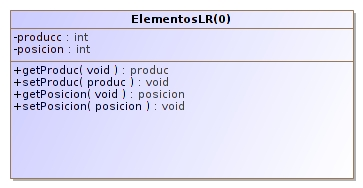
\includegraphics[scale=0.6]{figuras/Cap9/clase28.jpg}
% 	\caption{Representación gráfica de la clase ElementosLR(0).}
% 	\label{clase828}
%       \end{center}
%   \end{figure}

% \subsection{ElementosLR(1)}

% Esta clase representa al elemento LR(1) necesaria para llevar a cabo el análisis sintáctico ascendente LR-canónico. En la tabla \ref{tabla829} se recoge la especificación de la clase y en la figura \ref{clase829} se muestra su representación gráfica.


% \begin{longtable}[H]{|>{\columncolor[rgb]{0.63,0.79,0.95}}m{6cm} | m{8.5cm} |}
%  \caption{Clase ElementosLR(1)}

% \endfirsthead

% \multicolumn{2}{c}
% {{\tablename\ \thetable{} -- continúa de la página anterior}} \\
% \endhead

% \hline \multicolumn{2}{|r|}{{Continúa en la página siguiente}} \\ \hline
% \endfoot

% \hline
% \endlastfoot

% \hline
%  \textbf{Nombre} & \textbf{ElementosLR(1)}  \\ \hline
 
%  \textbf{Descripción} & Representa al elemento LR(1) necesaria en el análisis sintáctica ascendente LR-canónico.  \\ \hline
                       
%  \textbf{Atributos} & \begin{enumerate}
%  		\item  \textbf{produc}: este atributo representa el número de la producción que se está utilizando para la 				obtención de los elementos LR(1).
% 		\item \textbf{posicion}: este atributo representa la posición del punto en la parte derecha de la producción 			que se está utilizando.
% 		\item \textbf{anticipacion}: este atributo representa al símbolo de anticipación que es un símbolo no 					terminal o el símbolo \$.

% 	\end{enumerate} \\ \hline
 
%  \textbf{Métodos} & \begin{enumerate}
%  		\item \textbf{getProduc}: método público que permite obtener el número de la producción.
%  		\item \textbf{setProduc}: método público que permite asignar el valor del número de la producción que se 					está utilizando.
%  		\item \textbf{getPosicion}: método público que permite obtener la posición del punto dentro de la parte 					derecha de una producción.
%  		\item \textbf{setPosicion}: método público que permite asignar el valor de la posición del punto en la parte 			derecha 	de una producción.
%  		\item \textbf{getAnticipacion}: método público que permite obtener el símbolo de anticipación.
%  		\item \textbf{setAnticipacion}: método público que permite asignar el valor al símbolo de anticipación.
 		

% \end{enumerate}
                             
%  \label{tabla829}

% \end{longtable}

%  \begin{figure}[H]
%       \begin{center} 
% 	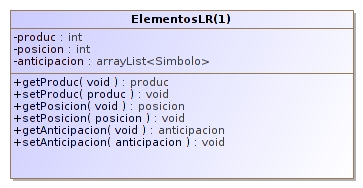
\includegraphics[scale=0.6]{figuras/Cap9/clase29.jpg}
% 	\caption{Representación gráfica de la clase ElementosLR(1).}
% 	\label{clase829}
%       \end{center}
%   \end{figure}
% \newpage
% \subsection{ElementosLALR(1)}

% Esta clase representa al elemento LALR(1) necesaria para llevar a cabo el análisis sintáctico ascendente LALR. En la tabla \ref{tabla830} se recoge la especificación de la clase y en la figura \ref{clase830} se muestra su representación gráfica.


% \begin{longtable}[H]{|>{\columncolor[rgb]{0.63,0.79,0.95}}m{6cm} | m{8.5cm} |}
%  \caption{Clase ElementosLALR(1)}

% \endfirsthead

% \multicolumn{2}{c}
% {{\tablename\ \thetable{} -- continúa de la página anterior}} \\
% \endhead

% \hline \multicolumn{2}{|r|}{{Continúa en la página siguiente}} \\ \hline
% \endfoot

% \hline
% \endlastfoot

% \hline
%  \textbf{Nombre} & \textbf{ElementosLALR(1)}  \\ \hline
 
%  \textbf{Descripción} & Representa al elemento LALR(1) necesaria en el análisis sintáctica ascendente LALR.  \\ \hline
                       
%   \textbf{Atributos} & \begin{enumerate}
%  		\item  \textbf{produc}: este atributo representa el número de la producción que se está utilizando para la 				obtención de los elementos LALR(1).
% 		\item \textbf{posicion}: este atributo representa la posición del punto en la parte derecha de la producción 			que se está utilizando.
% 		\item \textbf{anticipacion}: este atributo representa al símbolo de anticipación que es un símbolo no 					terminal o el símbolo \$.

% 	\end{enumerate} \\ \hline
 
%  \textbf{Métodos} & \begin{enumerate}
%  		\item \textbf{getProduc}: método público que permite obtener el número de la producción.
%  		\item \textbf{setProduc}: método público que permite asignar el valor del número de la producción que se 					está utilizando.
%  		\item \textbf{getPosicion}: método público que permite obtener la posición del punto dentro de la parte 					derecha de una producción.
%  		\item \textbf{setPosicion}: método público que permite asignar el valor de la posición del punto en la parte 			derecha 	de una producción.
%  		\item \textbf{getAnticipacion}: método público que permite obtener el símbolo de anticipación.
%  		\item \textbf{setAnticipacion}: método público que permite asignar el valor al símbolo de anticipación.
 		
% \end{enumerate}
                             
%  \label{tabla830}

% \end{longtable}

%  \begin{figure}[H]
%       \begin{center} 
% 	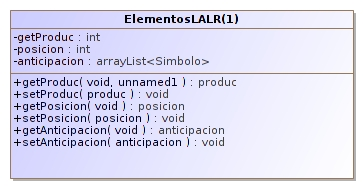
\includegraphics[scale=0.6]{figuras/Cap9/clase30.jpg}
% 	\caption{Representación gráfica de la clase ElementosLALR(1).}
% 	\label{clase830}
%       \end{center}
%   \end{figure}
  
% \subsection{Clase Simulador}

% Esta clase representa al simulador de gramáticas de contexto libre. En la tabla \ref{tabla811}
% se recoge la especificación de la clase y en la figura \ref{clase11} se muestra su representación gráfica.

% \begin{longtable}[H]{|>{\columncolor[rgb]{0.63,0.79,0.95}}m{6cm} | m{8.5cm} |}
%  \caption{Clase Simulador}

% \endfirsthead

% \multicolumn{2}{c}
% {{\tablename\ \thetable{} -- continúa de la página anterior}} \\
% \endhead

% \hline \multicolumn{2}{|r|}{{Continúa en la página siguiente}} \\ \hline
% \endfoot

% \hline
% \endlastfoot

% \hline
%  \textbf{Nombre} & \textbf{Simulador}  \\ \hline
 
%  \textbf{Descripción} & Representa a un simulador de gramáticas de contexto libre.  \\ \hline
                       
%  \textbf{Atributos} & \begin{enumerate}
% 		 \item \textbf{cadenaEntrada}: representa a la cadena de entrada, que estará compuesta por símbolos 			terminales y se usará  para ver si es reconocida o no durante la simulación.
% 		 \item \textbf{metodoSimulacion}: tipo enumerado que representa los dos tipos de simulaciones que se 						pueden llevar a cabo: método Descendente y método Ascendente.
%  		\item \textbf{modoFuncionamiento}: este tipo enumerado representa a la velocidad de funcionamiento del 					si\-mu\-la\-dor (paso a paso o contínuo).
 		
% 	\end{enumerate}\\ \hline
 
%  \textbf{Métodos} & \begin{enumerate}
%  		\item \textbf{cargarGramatica}: método público que permite seleccionar la gramática a ser simulada.
%  		\item \textbf{getMetodoSim}: método público que permite obtener el método de simulación, 1 si es el método 				descendente y 2 si es el método ascendente.
%  		\item \textbf{setMetodoSim}: método público que permite almacenar el valor del método de simulación, 1 si es 			el método descendente y 2 si es el método ascendente. 
%  		\item \textbf{getModoFunc}: método público que permite obtener el modo de funcionamiento del simulación, 1 				si es el modo contínuo y 2 si es el modo paso a paso.
%  		\item \textbf{setModoFunc}: método público que permite almacenar el valor del modo de funcionamiento del 					simulación, 1 si es el modo contínuo y 2 si es el modo paso a paso.
%  		\item \textbf{lanzarSimulador}: método privado que permite lanzar el simulador en función del método de 					funcionamiento y método de simulación seleccionado.  
%  		\item \textbf{generarInforme}: método público que permite obtener el informe de la simulación en formato 					PDF.
% 	\end{enumerate}
                                 
%  \label{tabla811}

% \end{longtable}

%  \begin{figure}[H]
%       \begin{center} 
% 	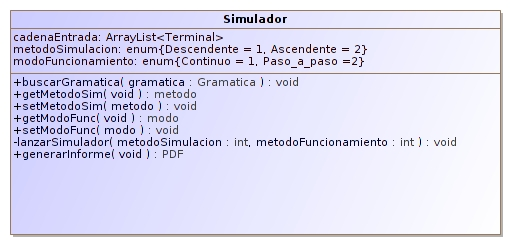
\includegraphics[scale=0.6]{figuras/Cap9/clase11.jpg}
% 	\caption{Representación gráfica de la clase Simulador.}
% 	\label{clase11}
%       \end{center}
%   \end{figure}
  
  
% \subsection{Clase CadenaEntrada}

% Esta clase representa a la cadena de entrada en la simulación de una gramática de contexto libre. En la tabla \ref{tabla821} se recoge la especificación de la clase y en la figura \ref{clase21} se muestra su representación gráfica.

% \begin{longtable}[H]{|>{\columncolor[rgb]{0.63,0.79,0.95}}m{6cm} | m{8.5cm} |}
%  \caption{Clase CadenaEntrada}

% \endfirsthead

% \multicolumn{2}{c}
% {{\tablename\ \thetable{} -- continúa de la página anterior}} \\
% \endhead

% \hline \multicolumn{2}{|r|}{{Continúa en la página siguiente}} \\ \hline
% \endfoot

% \hline
% \endlastfoot

% \hline
%  \textbf{Nombre} & \textbf{CadenaEntrada}  \\ \hline
 
%  \textbf{Descripción} & Representa la cadena de entrada en la simulación de una gramática de con\-tex\-to libre.  \\ \hline
                       
%  \textbf{Atributos} & \begin{enumerate}
%  		\item \textbf{cadena}: conjunto de símbolos terminales que forman parte de la cadena de entrada.
%  \end{enumerate} \\ \hline 
 
%  \textbf{Métodos} &  \begin{enumerate}
%  		\item \textbf{getCadena}: método público que recoge la cadena de entrada.
%  		\item \textbf{setCadena}: método público que modifica el valor de la cadena de entrada.
%  \end{enumerate}
                                 
%  \label{tabla821}

% \end{longtable}

%  \begin{figure}[H]
%       \begin{center} 
% 	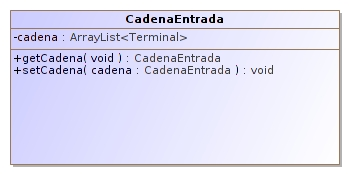
\includegraphics[scale=0.6]{figuras/Cap9/clase21.jpg}
% 	\caption{Representación gráfica de la clase CadenaEntrada.}
% 	\label{clase21}
%       \end{center}
%   \end{figure}


% \subsection{Clase ÁrbolSintáctico}

% Esta clase representa la creación de un nuevo objeto árbol sintáctico. Este árbol puede ser tanto descendente como ascendente y contendrá los siguientes métodos:

% \begin{longtable}[H]{|>{\columncolor[rgb]{0.63,0.79,0.95}}m{6cm} | m{8.5cm} |}
%  \caption{Clase ÁrbolSintáctico}\label{tabla-Clase-Arbol-Sintantico}

% \endfirsthead

% \multicolumn{2}{c}
% {{\tablename\ \thetable{} -- continúa de la página anterior}} \\
% \endhead

% \hline \multicolumn{2}{|r|}{{Continúa en la página siguiente}} \\ \hline
% \endfoot

% \hline
% \endlastfoot

% \hline
%  \textbf{Nombre} & \textbf{ÁrbolSintáctico}  \\ \hline
 
%  \textbf{Descripción} & Representa la generación de un árbol sintáctico, ya sea ascendente o descendente en la simulación de una gramática de con\-tex\-to libre.  \\ \hline
                       
%  \textbf{Atributos} & \begin{enumerate}
%  		\item \textbf{Grafo}: cadena que contiene la generación del grafo para añadirlo a un fichero de extensión .DOT.
%            \item \textbf{Gramática}: gramática a partir de la cual generar el grafo.
%           \item \textbf{Iterador}: iterador para controlar los pasos en la generación del árbol. 
%  \end{enumerate} \\ \hline 
 
%  \textbf{Métodos} &  \begin{enumerate}
%  		\item \textbf{getGrafo}: método público que recoge el grafo.
%  		\item \textbf{setGrafo}: método público que modifica el valor        del grafo.
%             \item \textbf{getGramática}: método público que recoge la gramática.
%  		\item \textbf{setGramática}: método público que modifica el valor        de la gramática.
%             \item \textbf{getIterador}: método público que recoge el iterador.
%  		\item \textbf{setIterador}: método público que modifica el valor        del iterador.
%             \item \textbf{generarImagenGrafo}: método público que permite la generación de una imagen usando un grafo.
%             \item \textbf{pintarGrafo}: método público que permite la representación en la ventana de la imagen del árbol.
%             \item \textbf{eliminarDirectorio}: método que permite realizar la eliminación de un directorio.
%             \item \textbf{guardarGrafoInicial}: método que permite generar el primer paso del árbol y almacenarlo en un .DOT. Es necesario tener en cuenta si el directorio existe o no para poder limpiarlo.
%             \item \textbf{guardarGrafoInicial}: método que permite generar cualquier paso del árbol y almacenarlo en un .DOT.
%  \end{enumerate}
                                 


% \end{longtable}

%  \begin{figure}[H]
%       \begin{center} 
% 	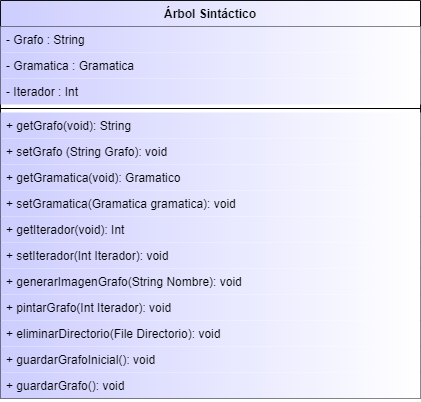
\includegraphics[scale=0.7]{figuras/Cap9/clase31.png}
% 	\caption{Representación gráfica de la clase ÁrbolSintáctico}
% 	\label{clase31}
%       \end{center}
%   \end{figure}


% \subsection{Clase Ayuda}

% Esta clase representa a la ayuda de la aplicación. En la tabla \ref{tabla815} se recoge la especificación de la clase y en la figura \ref{clase15} se muestra su representación gráfica.

% \begin{longtable}[H]{|>{\columncolor[rgb]{0.63,0.79,0.95}}m{6cm} | m{8.5cm} |}
%  \caption{Clase Ayuda}

% \endfirsthead

% \multicolumn{2}{c}
% {{\tablename\ \thetable{} -- continúa de la página anterior}} \\
% \endhead

% \hline \multicolumn{2}{|r|}{{Continúa en la página siguiente}} \\ \hline
% \endfoot

% \hline
% \endlastfoot

% \hline
%  \textbf{Nombre} & \textbf{Ayuda}  \\ \hline
 
%  \textbf{Descripción} & Representa a la ayuda de la aplicación.  \\ \hline
                       
%  \textbf{Atributos} & \begin{enumerate}
%  		\item \textbf{capitulos}: contiene el \textit{conjunto de capítulos} que forman la ayuda.
% 	\end{enumerate} \\ \hline
 
%  \textbf{Métodos} & \begin{enumerate}
%  		\item \textbf{inicializarAyuda}: método público que permite inicializar la ayuda. Es utilizado tanto por el 				editor como por el simulador.
%  		\item \textbf{buscarCapitulo}: método público que permite buscar un capítulo de la ayuda y recuperarlo.
%  		\item \textbf{visualizarCapitulo}: método público que permite visualizar un capítulo de la ayuda.
% 	\end{enumerate}
                             
%  \label{tabla815}

% \end{longtable}

%  \begin{figure}[H]
%       \begin{center} 
% 	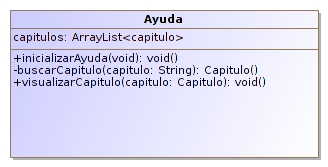
\includegraphics[scale=0.7]{figuras/Cap9/clase15.jpg}
% 	\caption{Representación gráfica de la clase Ayuda}
% 	\label{clase15}
%       \end{center}
%   \end{figure}

% \subsection{Clase Capitulo}

% Esta clase representa a los capítulos de la ayuda de la aplicación. En la tabla \ref{tabla816} se recoge la especificación de la clase y en la figura \ref{clase16} se muestra su representación gráfica.

% \begin{longtable}[H]{|>{\columncolor[rgb]{0.63,0.79,0.95}}m{6cm} | m{8.5cm} |}
%  \caption{Clase Capitulo}

% \endfirsthead

% \multicolumn{2}{c}
% {{\tablename\ \thetable{} -- continúa de la página anterior}} \\
% \endhead

% \hline \multicolumn{2}{|r|}{{Continúa en la página siguiente}} \\ \hline
% \endfoot

% \hline
% \endlastfoot

% \hline
%  \textbf{Nombre} & \textbf{Capitulo}  \\ \hline
 
%  \textbf{Descripción} & Representa a los capítulos de la ayuda de la aplicación.  \\ \hline
                       
%  \textbf{Atributos} & \begin{enumerate}
%  		\item \textbf{contenido}: \textit{contenido HTML} del capítulo.
% 		\end{enumerate} \\ \hline
 
%  \textbf{Métodos} & \begin{enumerate}
%  		\item \textbf{obtenerContenidoHTML}: método público que devuelve el contenido HTML del capítulo. Es 						utilizado por el módulo de la ayuda, para visualizar los capítulos de la misma.
% 	\end{enumerate}
                             
%  \label{tabla816}

% \end{longtable}

%  \begin{figure}[H]
%       \begin{center} 
% 	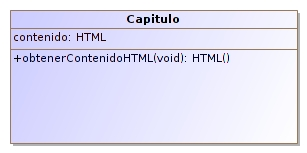
\includegraphics[scale=0.6]{figuras/Cap9/clase16.jpg}
% 	\caption{Representación gráfica de la clase Capitulo.}
% 	\label{clase16}
%       \end{center}
%   \end{figure}

% \subsection{Clase Tutorial}

% Esta clase representa al tutorial de la aplicación. En la tabla \ref{tabla817} se recoge la especificación de la clase y en la figura \ref{clase17} se muestra su representación gráfica.

% \begin{longtable}[H]{|>{\columncolor[rgb]{0.63,0.79,0.95}}m{6cm} | m{8.5cm} |}
%  \caption{Clase Tutorial}

% \endfirsthead

% \multicolumn{2}{c}
% {{\tablename\ \thetable{} -- continúa de la página anterior}} \\
% \endhead

% \hline \multicolumn{2}{|r|}{{Continúa en la página siguiente}} \\ \hline
% \endfoot

% \hline
% \endlastfoot

% \hline
%  \textbf{Nombre} & \textbf{Tutorial}  \\ \hline
 
%  \textbf{Descripción} & Representa al tutorial de la aplicación.  \\ \hline
                       
%  \textbf{Atributos} & \begin{enumerate}
%  		\item \textbf{lecciones}: lista de las lecciones del tutorial.
% 		\end{enumerate} \\ \hline
 
%  \textbf{Métodos} & \begin{enumerate}
%  		\item \textbf{visualizarLeccion}: método público que permite visualizar un lección del tutorial.
% 	\end{enumerate}
                             
%  \label{tabla817}

% \end{longtable}

% \begin{figure}[H]
%       \begin{center} 
% 	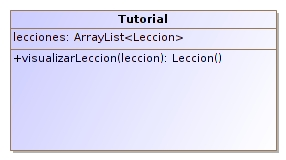
\includegraphics[scale=0.6]{figuras/Cap9/clase17.jpg}
% 	\caption{Representación gráfica de la clase Tutorial.}
% 	\label{clase17}
%       \end{center}
%   \end{figure}


% \subsection{Clase Leccion}

% Esta clase representa a las lecciones del tutorial de la aplicación. En la tabla \ref{tabla818} se recoge la especificación de la clase y en la figura \ref{clase18} se muestra su representación gráfica.

% \begin{longtable}[H]{|>{\columncolor[rgb]{0.63,0.79,0.95}}m{6cm} | m{8.5cm} |}
%  \caption{Clase Leccion}

% \endfirsthead

% \multicolumn{2}{c}
% {{\tablename\ \thetable{} -- continúa de la página anterior}} \\
% \endhead

% \hline \multicolumn{2}{|r|}{{Continúa en la página siguiente}} \\ \hline
% \endfoot

% \hline
% \endlastfoot

% \hline
%  \textbf{Nombre} & \textbf{Leccion}  \\ \hline
 
%  \textbf{Descripción} & Representa a las lecciones del tutorial de la aplicación.  \\ \hline
                       
%  \textbf{Atributos} & \begin{enumerate}
%  		\item \textbf{contenido}: contenido pdf de la lección.
% 		\end{enumerate} \\ \hline
 
%  \textbf{Métodos} & \begin{enumerate}
%  		\item \textbf{obtenerContenidoPDF}: método público que permite obtener el contenido PDF del la lección. 
% 	\end{enumerate}
                             
%  \label{tabla818}

% \end{longtable}

% \begin{figure}[H]
%       \begin{center} 
% 	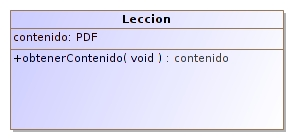
\includegraphics[scale=0.6]{figuras/Cap9/clase18.jpg}
% 	\caption{Representación gráfica de la clase Leccion.}
% 	\label{clase18}
%       \end{center}
%   \end{figure}
% \newpage

 \section{Relaciones entre las clases}

% En esta sección se rea\-li\-za\-rá un análisis de las relaciones existentes entre cada una de las clases analizadas anteriormente.

 \subsection{Componentes del sistema}

% Representa la relación de composición existente entre la clase principal de la aplicación, \textbf{SimAS} y las clases que representan a los componentes principales de la misma que son \textbf{Editor}, \textbf{Simulador}, \textbf{Ayuda} y \textbf{Tutorial}. En la figura \ref{rel1} se muestra la representación gráfica de esta relación.

%  \begin{figure}[H]
%       \begin{center} 
% 	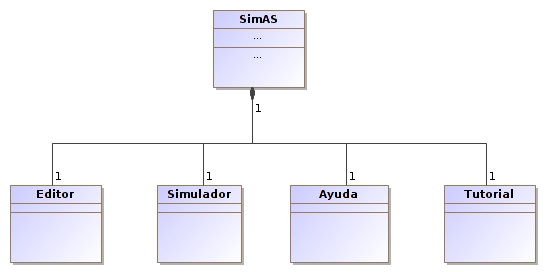
\includegraphics[scale=0.6]{figuras/Cap9/rel1.jpg}
% 	\caption{Relación de los componentes del Sistema.}
% 	\label{rel1}
%       \end{center}
%   \end{figure}

% \subsection{Relación Editor - Gramática}

% Representa la relación de uso existente entre el \textbf{editor} y la \textbf{gramática} de contexto libre, en las que el editor puede utilizar una gramáticas. En la figura \ref{rel2} se muestra la representación gráfica de esta relación.

%  \begin{figure}[H]
%       \begin{center} 
% 	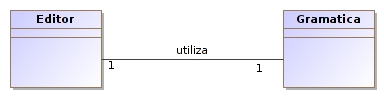
\includegraphics[scale=0.6]{figuras/Cap9/rel2.jpg}
% 	\caption{Relación Editor-Gramatica.}
% 	\label{rel2}
%       \end{center}
%   \end{figure}


% \subsection{Relación Simulador - Gramática}

% Representa la relación de uso existente entre el \textbf{si\-mu\-la\-dor} y la \textbf{gramática} de contexto libre, en las que el si\-mu\-la\-dor puede utilizar una gramática. En la figura \ref{rel3} se muestra la representación gráfica de esta relación.

% \begin{figure}[H]
%       \begin{center} 
% 	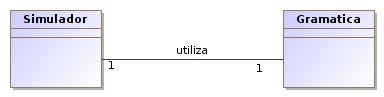
\includegraphics[scale=0.6]{figuras/Cap9/rel3.jpg}
% 	\caption{Relación Simulador-Gramatica.}
% 	\label{rel3}
%       \end{center}
%   \end{figure}

% \subsection{Relación Ayuda - Capitulo}

% Representa la relación de composición existente entre la \textbf{ayuda} del simulador y los \textbf{capítulos}, que representa el hecho de que la ayuda se compone de uno o varios capítulos. En la figura \ref{rel4} se muestra la representación gráfica de esta relación.

% \begin{figure}[H]
%       \begin{center} 
% 	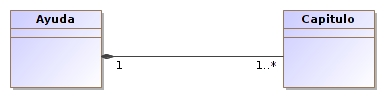
\includegraphics[scale=0.6]{figuras/Cap9/rel4.jpg}
% 	\caption{Relación Ayuda-Capitulo.}
% 	\label{rel4}
%       \end{center}
%   \end{figure}

% \subsection{Relación Tutorial - Leccion}

% Representa la relación de composición existente entre el \textbf{tutorial} del simulador y las \textbf{lecciones}, que representa el hecho de que el tutorial se compone de una o varias lecciones. En la figura \ref{rel5} se muestra la representación gráfica de esta relación.

% \begin{figure}[H]
%       \begin{center} 
% 	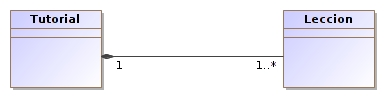
\includegraphics[scale=0.6]{figuras/Cap9/rel5.jpg}
% 	\caption{Relación Tutorial-Leccion.}
% 	\label{rel5}
%       \end{center}
%   \end{figure}

% \subsection{Componentes de la gramática}

% Representa la relación de composición existente entre la \textbf{gramática} y sus componentes (\textbf{produccion}, \textbf{NoTerminal} y \textbf{Terminal}). La gramática se compone de varias producciones, de uno o varios símbolos no terminales y uno o varios símbolos terminales. En la figura \ref{rel6} se muestra la representación gráfica de esta relación.

% \begin{figure}[H]
%       \begin{center} 
% 	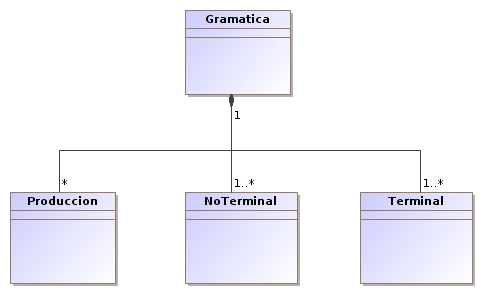
\includegraphics[scale=0.6]{figuras/Cap9/rel6.jpg}
% 	\caption{Relación componentes de la Gramatica.}
% 	\label{rel6}
%       \end{center}
%   \end{figure}
  
% \subsection{Gramatica - TablaPredictiva}

% Representa la relación existente entre la \textbf{gramática} y la \textbf{tabla predictiva}, de forma que de una gramática se puede obtener ninguna o una tabla predictiva, mientras que una tabla predictiva solamente puede pertenecer a una única gramática. En la figura \ref{rel7} se muestra la representación gráfica de esta relación.

% \begin{figure}[H]
%       \begin{center} 
% 	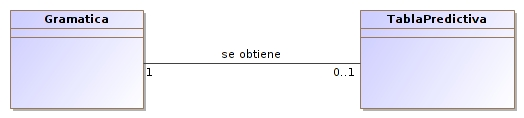
\includegraphics[scale=0.6]{figuras/Cap9/rel7.jpg}
% 	\caption{Relación Gramatica-TablaPredictiva.}
% 	\label{rel7}
%       \end{center}
%   \end{figure}

% \subsection{Gramatica - TablaLR}

% Representa la relación existente entre la \textbf{gramática} y la \textbf{tabla LR}, de forma que de una gramática se puede obtener ninguna o tres tablas LR (una por cada método de análisis sintáctico ascendente), mientras que una tabla LR solamente puede pertenecer a una única gramática. En la figura \ref{rel8} se muestra la representación gráfica de esta relación.

% \begin{figure}[H]
%       \begin{center} 
% 	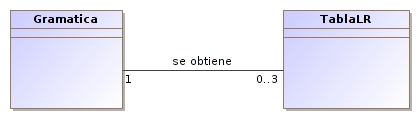
\includegraphics[scale=0.6]{figuras/Cap9/rel8.jpg}
% 	\caption{Relación Gramatica-TablaLR.}
% 	\label{rel8}
%       \end{center}
%   \end{figure}
  
% \subsection{TablaPredictiva - FuncionError}

% Representa la relación existente entre la \textbf{tabla Predictiva} y las \textbf{funciones de e\-rror}, de forma que una tabla Predictiva podrá ser completada con ninguna o varias función de e\-rror. En la figura \ref{rel9} se muestra la representación gráfica de esta relación.
  
%  \begin{figure}[H]
%       \begin{center} 
% 	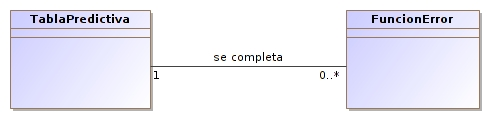
\includegraphics[scale=0.6]{figuras/Cap9/rel9.jpg}
% 	\caption{Relación TablaPredictiva-FuncionError.}
% 	\label{rel9}
%       \end{center}
%   \end{figure}
  
% \subsection{Componentes de la tabla LR}

% Representa la relación de composición existente entre la \textbf{tabla LR} y sus componentes (\textbf{ParteIrA} y \textbf{ParteAccion}). La tabla LR se compone de una parte acción y una parte ir\_a. En la figura \ref{rel16} se muestra la representación gráfica de esta relación.

%  \begin{figure}[H]
%       \begin{center} 
% 	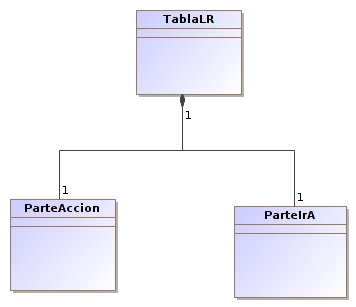
\includegraphics[scale=0.6]{figuras/Cap9/rel16.jpg}
% 	\caption{Relación componentes de la tabla LR}
% 	\label{rel16}
%       \end{center}
%   \end{figure}
  
% \subsection{Relación ParteAccion - FuncionError}

% Representa la relación existente entre la \textbf{parte acción} de la tabla LR y las \textbf{funciones de e\-rror}, de forma que la parte acción podrá ser completada con ninguna o varias función de e\-rror. En la figura \ref{rel10} se muestra la representación gráfica de esta relación.
  
%  \begin{figure}[H]
%       \begin{center} 
% 	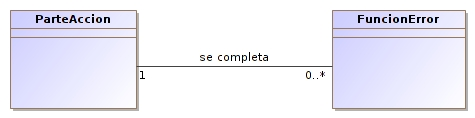
\includegraphics[scale=0.6]{figuras/Cap9/rel10.jpg}
% 	\caption{Relación ParteAccion-FuncionError.}
% 	\label{rel10}
%       \end{center}
%   \end{figure}
  
% \subsection{Relación Simulador - CadenaEntrada}

% Representa la relación existente entre el \textbf{simulador} y la \textbf{cadena de entrada}, de forma que el simulador tiene una sola cadena de entrada y ésta solamente pertenece a un simulador. En la figura \ref{rel17} se muestra la representación gráfica de esta relación.
  
%  \begin{figure}[H]
%       \begin{center} 
% 	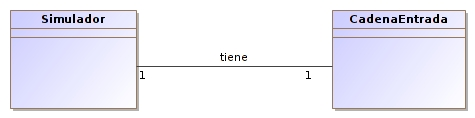
\includegraphics[scale=0.6]{figuras/Cap9/rel17.jpg}
% 	\caption{Relación Simulador - CadenaEntrada.}
% 	\label{rel17}
%       \end{center}
%   \end{figure}
  
% \subsection{Relación de especialización de los símbolos}

% Representa la relación de herencia o especialización de los símbolos de la gramática, que se especializan de la clase \textbf{Simbolo} a las clases \textbf{Terminal} y \textbf{NoTerminal}. De esta forma, los símbolos de la gramática podrán ser Terminales o NoTerminales, teniendo así la gramática una colección de símbolos terminales y no terminales, sin ningún límite en cuanto a la cantidad de los mismos. En la figura \ref{rel11} se muestra la representación gráfica de esta relación.
  
%   \begin{figure}[H]
%       \begin{center} 
% 	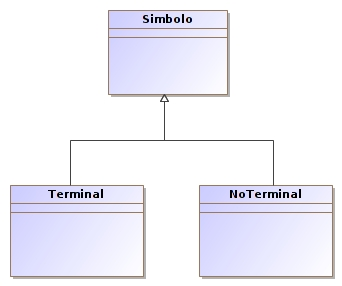
\includegraphics[scale=0.6]{figuras/Cap9/rel11.jpg}
% 	\caption{Relación de los símbolos de la gramática.}
% 	\label{rel11}
%       \end{center}
%   \end{figure}
  
% \subsection{Relación de composición de las producciones}

% Representa la relación de composición de las producciones de la gramática. Esta relación indica que las producciones se componen de un \textbf{Antecedente} y un \textbf{Consecuente}. En la figura \ref{rel12} se muestra la representación gráfica de esta relación.
  
%    \begin{figure}[H]
%       \begin{center} 
% 	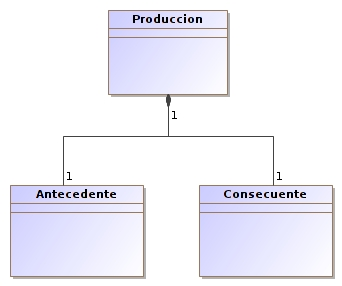
\includegraphics[scale=0.6]{figuras/Cap9/rel12.jpg}
% 	\caption{Relación de las producciones de la gramática.}
% 	\label{rel12}
%       \end{center}
%   \end{figure}
  
  
% \subsection{Relación Antecedente - NoTerminal}

% Representa la relación existente entre el \textbf{antecedente} y un símbolo \textbf{no terminal}. Esta relación implica que el antecedente contendrá un único símbolo no terminal, pero que un símbolo no terminal podrá estar contenido en varios antecedentes de diferentes producciones. En la figura \ref{rel14} se muestra la representación gráfica de esta relación.  
  
%   \begin{figure}[H]
%       \begin{center} 
% 	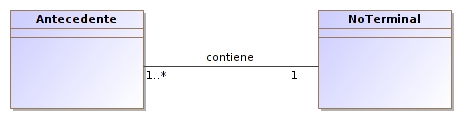
\includegraphics[scale=0.6]{figuras/Cap9/rel14.jpg}
% 	\caption{Relación Antecendente-NoTerminal.}
% 	\label{rel14}
%       \end{center}
%   \end{figure}
  
% \subsection{Relación Consecuente - Simbolo}

% Representa la relación existente entre el \textbf{consecuente} y los \textbf{símbolos} de la gramática. Esta relación implica que el consecuente contendrá uno o varios símbolos. Además, esta relación representa el hecho de que un símbolo podrá estar contenido en más de un consecuente (en distintas producciones).  En la figura \ref{rel15} se muestra la representación gráfica de esta relación.
  
%    \begin{figure}[H]
%       \begin{center} 
% 	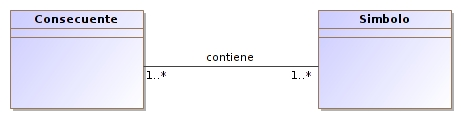
\includegraphics[scale=0.6]{figuras/Cap9/rel15.jpg}
% 	\caption{Relación Consecuente-Simbolo.}
% 	\label{rel15}
%       \end{center}
%   \end{figure}
  
% \subsection{Relación Terminal - CadenaEntrada.}

% Representa la relación existente entre un símbolo \textbf{terminal} y la \textbf{cadena de entrada}. Esta relación implica que la cadena de entrada está formada por uno o varios símbolos terminales. En la figura \ref{rel13} se muestra la representación gráfica de esta relación.
  
%    \begin{figure}[H]
%       \begin{center} 
% 	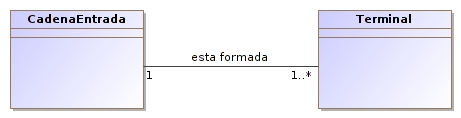
\includegraphics[scale=0.6]{figuras/Cap9/rel13.jpg}
% 	\caption{Relación Terminal - CadenaEntrada.}
% 	\label{rel13}
%       \end{center}
%   \end{figure}
  
% \subsection{Componentes de la gramática II}

% Representa otra relación de composición existente entre la \textbf{gramática} y sus componentes (\textbf{colección canónica LR(0)}, \textbf{colección canónica LR(1)} y \textbf{colección canónica LALR (1)}). La gramática se compone de una una colección canónica LR(0), de una colección canónica LR(1) y de una colección canónica LALR(1). En la figura \ref{rel18} se muestra la representación gráfica de esta composición.

%  \begin{figure}[H]
%       \begin{center} 
% 	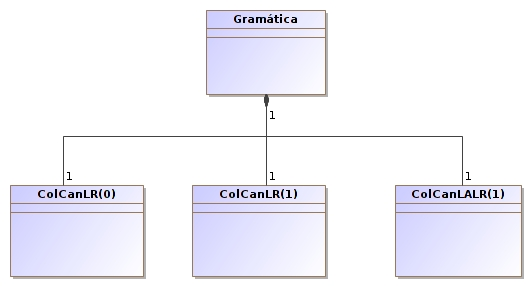
\includegraphics[scale=0.6]{figuras/Cap9/rel18.jpg}
% 	\caption{Relación componentes de la gramática II.}
% 	\label{rel18}
%       \end{center}
%   \end{figure}
  
% \subsection{Relación ColCanLR(0) - ConjElementosLR(0)}

% Representa la relación existente entre la \textbf{colección canónica LR(0)} y el \textbf{conjunto de elementos LR(0)}. Esta relación implica que la colección canónica LR(0) esta formada por uno o varios conjuntos de elementos LR(0). En la figura \ref{rel19} se muestra la representación gráfica de esta relación.
  
%    \begin{figure}[H]
%       \begin{center} 
% 	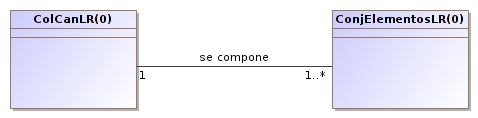
\includegraphics[scale=0.6]{figuras/Cap9/rel19.jpg}
% 	\caption{Relación ColCanLR(0) - ConjElementosLR(0)}
% 	\label{rel19}
%       \end{center}
%   \end{figure}
  
% \subsection{Relación ColCanLR(1) - ConjElementosLR(1)}

% Representa la relación existente entre la \textbf{colección canónica LR(1)} y el \textbf{conjunto de elementos LR(1)}. Esta relación implica que la colección canónica LR(1) esta formada por uno o varios conjuntos de elementos LR(1). En la figura \ref{rel20} se muestra la representación gráfica de esta relación.
  
%    \begin{figure}[H]
%       \begin{center} 
% 	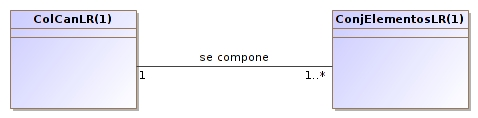
\includegraphics[scale=0.6]{figuras/Cap9/rel20.jpg}
% 	\caption{Relación ColCanLR(1) - ConjElementosLR(1).}
% 	\label{rel20}
%       \end{center}
%   \end{figure}
  
% \subsection{Relación ColCanLALR(1) - ConjElementosLALR(1)}

% Representa la relación existente entre la \textbf{colección canónica LALR(1)} y el \textbf{conjunto de elementos LALR(1)}. Esta relación implica que la colección canónica LALR(1) esta formada por uno o varios conjuntos de elementos LALR(1). En la figura \ref{rel21} se muestra la representación gráfica de esta relación.
  
%    \begin{figure}[H]
%       \begin{center} 
% 	\includegraphics[scale=0.6]{figuras/Cap9/rel21.jpg}
% 	\caption{Relación ColCanLALR(1) - ConjElementosLALR(1).}
% 	\label{rel21}
%       \end{center}
%   \end{figure}
  
% \subsection{Relación ConjElementosLR(0) - ElementosLR(0)}

% Representa la relación existente entre el \textbf{conjunto de elementos LR(0)} y los \textbf{elementos LR(0)}. Esta relación implica que el conjunto de elementos LR(0) esta formada por uno o varios elementos LR(0). En la figura \ref{rel22} se muestra la representación gráfica de esta relación.
  
%    \begin{figure}[H]
%       \begin{center} 
% 	\includegraphics[scale=0.6]{figuras/Cap9/rel22.jpg}
% 	\caption{Relación ConjElementosLR(0) - ElementosLR(0).}
% 	\label{rel22}
%       \end{center}
%   \end{figure}
  
% \subsection{Relación ConjElementosLR(1) - ElementosLR(1)}

% Representa la relación existente entre el \textbf{conjunto de elementos LR(1)} y los \textbf{elementos LR(1)}. Esta relación implica que el conjunto de elementos LR(1) esta formada por uno o varios elementos LR(1). En la figura \ref{rel23} se muestra la representación gráfica de esta relación.
  
%    \begin{figure}[H]
%       \begin{center} 
% 	\includegraphics[scale=0.6]{figuras/Cap9/rel23.jpg}
% 	\caption{Relación ConjElementosLR(1) - ElementosLR(1).}
% 	\label{rel23}
%       \end{center}
%   \end{figure}
  
% \subsection{Relación ConjElementosLALR(1) - ElementosLALR(1)}

% Representa la relación existente entre el \textbf{conjunto de elementos LALR(1)} y los \textbf{elementos LALR(1)}. Esta relación implica que el conjunto de elementos LALR(1) esta formada por uno o varios elementos LALR(1). En la figura \ref{rel24} se muestra la representación gráfica de esta relación.
  
%    \begin{figure}[H]
%       \begin{center} 
% 	\includegraphics[scale=0.6]{figuras/Cap9/rel24.jpg}
% 	\caption{Relación ConjElementosLALR(1) - ElementosLALR(1).}
% 	\label{rel24}
%       \end{center}
%   \end{figure}
  
% \subsection{Relación ElementosLR(0) - Producción}

% Representa la relación existente entre los \textbf{elementos LR(0)} y las \textbf{producciones}. Esta relación implica que los elementos LR(0) se obtienen de una producción y, además, que de una producción se pueden obtener uno o varios elementos LR(0). En la figura \ref{rel25} se muestra la representación gráfica de esta relación.
  
%    \begin{figure}[H]
%       \begin{center} 
% 	\includegraphics[scale=0.6]{figuras/Cap9/rel25.jpg}
% 	\caption{Relación ElementosLR(0) - Producción.}
% 	\label{rel25}
%       \end{center}
%   \end{figure}
  
% \subsection{Relación ElementosLR(1) - Producción}

% Representa la relación existente entre los \textbf{elementos LR(1)} y las \textbf{producciones}. Esta relación implica que los elementos LR(1) se obtienen de una producción y, además, que de una producción se pueden obtener uno o varios elementos LR(1). En la figura \ref{rel26} se muestra la representación gráfica de esta relación.
  
%    \begin{figure}[H]
%       \begin{center} 
% 	\includegraphics[scale=0.6]{figuras/Cap9/rel26.jpg}
% 	\caption{Relación ElementosLR(1) - Producción.}
% 	\label{rel26}
%       \end{center}
%   \end{figure}
  
% \subsection{Relación ElementosLALR(1) - Producción}

% Representa la relación existente entre los \textbf{elementos LALR(1)} y las \textbf{producciones}. Esta relación implica que los elementos LALR(1) se obtienen de una producción y, además, que de una producción se pueden obtener uno o varios elementos LALR(1). En la figura \ref{rel27} se muestra la representación gráfica de esta relación.
  
%    \begin{figure}[H]
%       \begin{center} 
% 	\includegraphics[scale=0.6]{figuras/Cap9/rel27.jpg}
% 	\caption{Relación ElementosLALR(1) - Producción.}
% 	\label{rel27}
%       \end{center}
%   \end{figure}
  
  
 \section{Diagrama de clases del sistema}

% A continuación, en la siguiente figura \ref{clases} se recoge el diagrama de clases del sistema, según las especificaciones realizadas hasta este punto.

% \newpage
%  \begin{figure}[H]
%       \begin{center} 
% 	\includegraphics[angle=90, scale=0.30]{figuras/Cap9/clases.png}
% 	\caption{Diagrama de clases.}
% 	\label{clases}
%       \end{center}
%   \end{figure}
